\documentclass[12pt,a4paper]{article}

%% -------------------------------
%% NCI Large Project Template      
%% -------------------------------



%% ---------------------------------
%% |      Additional packages      |
%% ---------------------------------
%% 

\usepackage[a4paper, margin=1in]{geometry} %% margins
\usepackage{graphicx} %http://en.wikibooks.org/wiki/LaTeX/Importing_Graphics#Graphics_storage
\usepackage[export]{adjustbox}
\usepackage[svgnames]{xcolor}
\usepackage[absolute,overlay]{textpos}
\usepackage{longtable}
\usepackage{tikz}
\usepackage{enumitem}
\usepackage{natbib} %for harvard style refs
\usepackage{booktabs,tabularx} % marksheet
\usepackage{algorithm} % Code-Listings
\usepackage{algorithmic} % Code-Listings
\usepackage{amssymb} %check list
\usepackage{pdflscape} %for logical data map
% see http://www.ctan.org/tex-archive/macros/latex/contrib/algorithm2e/algorithm2e.pdf
% for more sophisticated algorithm listings
\usepackage[a4paper,bookmarks=true, colorlinks=false]{hyperref} % Links - must be last package
\usepackage{listings} % R code listings
\usepackage{lipsum} % dummy text

% Formatting for R code
\lstset{language=R,
    basicstyle=\small\ttfamily,
    stringstyle=\color{DarkGreen},
    otherkeywords={0,1,2,3,4,5,6,7,8,9},
    morekeywords={TRUE,FALSE},
    deletekeywords={data,frame,length,as,character},
    keywordstyle=\color{blue},
    commentstyle=\color{DarkGreen},
}

\DeclareGraphicsExtensions{.pdf,.png,.jpg}
\graphicspath{{./figures/}} %Use curly braces for each path to add 

%% ---------------------------------
%% | Information about the report  |
%% ---------------------------------

%Change these specific for your project
\newcommand{\myname}{Forename Surname}
\newcommand{\SID}{1234567}
\newcommand{\mytopic}{Insert Title Here}

%Uncomment as appropriate
\newcommand{\lecturer}{Dr. Simon Caton}
%\newcommand{\lecturer}{Dr. Horacio Gonz\'{a}lez--V\'{e}lez}
%\newcommand{\lecturer}{Dr. Pierpaolo Dondio}
%\newcommand{\lecturer}{Noel Cosgrave}


%% ---------------------------------
%% |       DO NOT CHANGE THIS       |
%% ---------------------------------
\newcommand{\duedate}{26/11/2018}

%% -------------------------------
%% |  Information for PDF file   |
%% -------------------------------
%% Auto-Fill this information
\hypersetup{
 pdfauthor={\myname},
 pdftitle={\mytopic},
 pdfsubject={DWBI Project}
}


% Describe separation hints here:
\hyphenation{
% Man-age-ment
}

%%%%%%%%%%%%%%%%%%%%%%%%%%%%%%%%%
%% Here, main documents begins %%
%%%%%%%%%%%%%%%%%%%%%%%%%%%%%%%%%
\begin{document}

%% titlepage.tex
%%

% coordinates for the bg shape on the titlepage
\newcommand{\diameter}{20}
\newcommand{\xone}{-15}
\newcommand{\xtwo}{160}
\newcommand{\yone}{15}
\newcommand{\ytwo}{-253}
\newcommand{\myinstitute}{School of Computing \\ National College of Ireland}

\begin{titlepage}
% bg shape
\begin{tikzpicture}[overlay]
\draw[color=gray]  
 		 (\xone mm, \yone mm)
  -- (\xtwo mm, \yone mm)
 arc (90:0:\diameter pt) 
  -- (\xtwo mm + \diameter pt , \ytwo mm) 
	-- (\xone mm + \diameter pt , \ytwo mm)
 arc (270:180:\diameter pt)
	-- (\xone mm, \yone mm);
\end{tikzpicture}
	\begin{textblock}{10}[0,0](7.75,1)
		
\includegraphics[width=.3\textwidth, center]{logos/NCI_Logo_colour.jpg}
	\end{textblock}	
	\vspace*{5.5cm}
	\begin{center}
		\Huge{Data Warehousing and Business Intelligence Project}\\
		\vspace*{1cm}
		\small{on}\\
		\vspace*{1cm}
		\Large{
			\mytopic
		}\\
		\vspace*{2cm}
		\huge{\myname}\\
		\Large{\SID}\\
		
		\vspace*{4.5cm}
		\large{MSc/PGDip Data Analytics -- 2018/9}\\
		\vspace*{2cm}
		\large{Submitted to: \lecturer}
	\end{center}

\end{titlepage}


\pagestyle{empty}

	\begin{textblock}{10}[0,0](7.75,1)
		
\includegraphics[width=.3\textwidth, center]{logos/NCI_Logo_colour.jpg}
	\end{textblock}

\begin{center}
\textbf{National College of Ireland}\\

\textbf{Project Submission Sheet -- 2017/2018}\\

\textbf{School of Computing}
\end{center}

\begin{table}[htbp]
\begin{center}
\begin{tabular}{||p{.25\textwidth}|p{.7\textwidth}||}
\hline
\textbf{Student Name:}& \myname \\\hline
\textbf{Student ID:}& \SID \\\hline 
\textbf{Programme:}& MSc Data Analytics \\\hline
\textbf{Year:}&  2018/9 \\\hline
\textbf{Module:} & Data Warehousing and Business Intelligence \\\hline
\textbf{Lecturer:}& \lecturer \\\hline
\textbf{Submission Due Date:}& \duedate \\\hline
\textbf{Project Title:}& \mytopic \\\hline 
\end{tabular}
\end{center}
\end{table}
\vspace{-.5cm}
I hereby certify that the information contained in this (my submission) is information pertaining to my own individual work that I conducted for this project. All information other than my own contribution is fully and appropriately referenced and listed in the relevant bibliography section. I assert that I have not referred to any work(s) other than those listed. I also include my TurnItIn report with this submission.

\underline {\textbf{ALL}} materials used must be referenced in the bibliography section. Students are encouraged to use the Harvard Referencing Standard supplied by the Library. To use other author's written or electronic work is an act of plagiarism and may result in disciplinary action. Students may be required to undergo a viva (oral examination) if there is suspicion about the validity of their submitted work.

\begin{table}[htbp]
\begin{center}
\begin{tabular}{||p{.25\textwidth}|p{.7\textwidth}||}
\hline
\textbf{Signature:}& \\
 & \\\hline 
\textbf{Date:}& \today  \\\hline

\end{tabular}
\end{center}
\end{table}

\vspace{-.5cm}
\textbf{PLEASE READ THE FOLLOWING INSTRUCTIONS:}\\
1. Please attach a completed copy of this sheet to each project (including
multiple copies).\\
2. \textbf{You must ensure that you retain a HARD COPY of ALL projects},
both for your own reference and in case a project is lost or mislaid. It is
not sufficient to keep a copy on computer. Please do not bind projects or
place in covers unless specifically requested.\\
3. Assignments that are submitted to the Programme Coordinator office must be
placed into the assignment box located outside the office.

\begin{table}[htbp]
\begin{center}
\begin{tabular}{||p{.25\textwidth}|p{.7\textwidth}||}
\hline
\multicolumn{2}{||l||}{\textbf{Office Use Only}} \\\hline
Signature:& \\
~ & \\\hline
Date:& \\\hline
Penalty Applied (if applicable):& \\\hline
\end{tabular}
\end{center}
\end{table}

\newcommand{\criteria}[2]{& & \\ & & \\ #1 & of #2 & \\ & & \\ & & \\\hline}
\newcommand{\total}[1]{\hline\hline  & & \\ Total & of #1 & \\ & &  \\\hline\hline}

\begin{table}[h]
\centering
\caption{Mark sheet -- do not edit}
\begin{tabular}{||l|r|p{10cm}||}
\hline\hline
Criteria & Mark Awarded & Comment(s) \\
\hline\hline
\criteria{Objectives}{5}
\criteria{Related Work}{10}
\criteria{Data}{25}
\criteria{ETL}{20}
\criteria{Application}{30}
\criteria{Video}{10}
\criteria{Presentation}{10}
\hline
\total{100}
\hline
\end{tabular}
\end{table}





\section*{Project Check List}

This section capture the core requirements that the project entails represented as a check list for convenience.


%% 
% Use: \item[$\boxtimes$] 
% To denote a that you have checked an item!
%%

\begin{itemize}
\item[$\boxtimes$] Used \LaTeX \ template
\item[$\square$] Three Business Requirements listed in introduction
\item[$\square$] At least one structured data source
\item[$\square$] At least one unstructured data source
\item[$\square$] At least three sources of data
\item[$\square$] Described all sources of data
\item[$\square$] All sources of data are less than one year old, i.e. released after 17/09/2017 
\item[$\square$] Inserted and discussed star schema
\item[$\square$] Completed logical data map
\item[$\square$] Discussed the high level ETL strategy
\item[$\square$] Provided 3 BI queries
\item[$\square$] Detailed the sources of data used in each query
\item[$\square$] Discussed the implications of results in each query
\item[$\square$] Reviewed at least 5-10 appropriate papers on topic of your DWBI project

\end{itemize}


%% -----------------
%% |   Main part   |
%% -----------------

\title{\mytopic}%
\author{\myname \\ \SID}%
\date{\today}
\maketitle

\pagenumbering{arabic}
\begin{abstract}
Abstract goes here. You should provide a high-level (approx. 150 -- 250 words) overview of your project, its motivation, and the core objectives / business requirements addressed.
\end{abstract}
%% introduction.tex
%%

%% ==============================
\section{Introduction}
\label{sec:Introduction}
%% ==============================

In this section you need to motivate your project (using citations). Why are you doing it? You should articulate the business requirements that your project seeks to address as motivation. These should be quantifiable and addressed via the BI Queries in Section~\ref{sec:BIQueries}.

Lorem ipsum dolor sit amet, ut veri deleniti eloquentiam sea~\cite{FengB16}. Ea commodo aperiam complectitur pri, usu et case dolore. \cite{KuneKARB16} ad quidam regione percipitur, est ut possit bonorum persecuti. Quis utinam offendit eu usu, eu accumsan disputando per, id cibo reprehendunt sit~\cite{BeloglazovB15,GomesCT15}. In melius legendos corrumpit pro. Eos dico dignissim voluptatibus et, duo nisl cibo ut. Diceret periculis posidonium cum eu. \cite{GomesCT15} regione nam ex. Vix id viris phaedrum. Pri augue cetero probatus ut.

\begin{enumerate}[label=(Req-\arabic*)]
\item my first requirement
\item my second requirement
\item \ldots
\end{enumerate}
\section{Data Sources}
\label{sec:dataSources}
Here you should present and formally describe your sources of data used in the project.

\begin{table}
\centering
\begin{tabular}[h]{||p{.2\linewidth}||p{.2\linewidth}|p{.5\linewidth}||}
\hline\hline
Source & Type & Brief Summary \\\hline\hline

Kaggle & Structured & Used because I was too lazy to get a difficult dataset \\\hline
Data.world & Structured & Basically provides the same data as the above, but I'm hoping no one will notice \\\hline
Twitter & Unstructured & I didn't know what else to do and can't think for myself. \\\hline\hline
\end{tabular}

\caption{Summary of sources of data used in the project}

\end{table}

\subsection{Source 1: Kaggle}
The kaggle movies dataset downloaded this source from: \url{https://www.kaggle.com/tmdb/tmdb-movie-metadata#tmdb_5000_movies.csv}  provides 20 columns of information on 5000 movies. 

These are \ldots . 

However, relevant to this project are: \ldots

This dataset addresses the business requirements listed in Section \ref{sec:Introduction} in the following ways \ldots

\subsection{Source 2: \ldots}
\ldots

\subsection{Source 3: \ldots}
\ldots



\section{Related Work}
\label{sec:rw}

In this section, discuss related work on your topic of choice. Consider answering the following questions:

\begin{enumerate}[label=Q\arabic*]
\item How have these (or similar) datasets been used before?
\item What is generally known about the domain within which your requirements (in Section~\ref{sec:Introduction}) are situated?
\item What significant results exist in this area, and how to you expect to add to them by undertaking this project?
\end{enumerate}

See \cite{hall2018editorial} for an example of a lit review that looks at specific challenges and approaches within a given area.
\section{Data Model}
\label{sec:dataModel}

In this section, provide details of your dimensions, why they are in your data model, how sources of data contribute to each of the dimensions, and present your star schema. 

Do not do this:

\begin{figure}[ht]
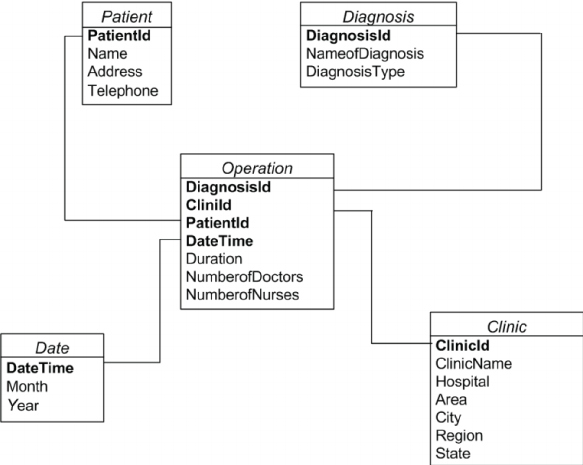
\includegraphics[scale=\textwidth]{figures/sampleStar.png}
\caption{Some star schema i found online}
\label{fig:star}
\end{figure}

So i have 4 dimensions, as seen in \figurename~\ref{fig:star}. They are good and answer all the queries. I was lazy, so i took a screen shot of SSAS, which my lecturer cannot read.

Instead, provide a detailed discussion on the composition of each dimension, justifying its contents and any hierarchies you have designed in to facilitate drill down. It's seriously unlikely that you can map a dataset 1 to 1 with all columns to a dimension, so explain here which components of which dataset map to which dimension. For the fact table, be precise with respect to the granularity of the facts, and motivate each fact included linking it to at least one of your requirements.
\begin{landscape}
\section{Logical Data Map}
\label{sec:map}

In this section, describe your logical data map, i.e. how every row of every data source is handled such that it is a part of your star schema.

\begin{center}
\begin{longtable}{|*5{p{.1\linewidth}|}p{.4\linewidth}|}
    \caption{Logical Data Map describing all transformations, sources and destinations for all components of the data model illustrated in \figurename~\ref{fig:star}}\\
    \hline\hline
    {\bf Source} & {\bf Column} & {\bf Destination} & {\bf Column} & {\bf Type} & {\bf Transformation} \\ \hline\hline
    \endfirsthead
\multicolumn{6}{c}%
	{\tablename\ \thetable\ -- \textit{Continued from previous page}} \\
	\hline
	{\bf Source} & {\bf Column} & {\bf Destination} & {\bf Column} & {\bf Type} & {\bf Transformation}  \\
	\hline
	\endhead
	\hline \multicolumn{6}{r}{\textit{Continued on next page}} \\
	\endfoot
	\hline
	\endlastfoot

% rows begin here:

    1 & Movie Genre & DimMovie & Genre & Dimension & Primary Genre (1st one) only, all characters after first comma removed \\\hline
    1 & Revenue & FactTable & Revenue & Fact & Rounded to nearest million \$ \\\hline
    1 & Movie Genre & DimMovie & Genre & Dimension & Primary Genre (1st one) only, all characters after first comma removed \\\hline
    1 & Revenue & FactTable & Revenue & Fact & Rounded to nearest million \$ \\\hline
        1 & Movie Genre & DimMovie & Genre & Dimension & Primary Genre (1st one) only, all characters after first comma removed \\\hline
    1 & Revenue & FactTable & Revenue & Fact & Rounded to nearest million \$ \\\hline
        1 & Movie Genre & DimMovie & Genre & Dimension & Primary Genre (1st one) only, all characters after first comma removed \\\hline
    1 & Revenue & FactTable & Revenue & Fact & Rounded to nearest million \$ \\\hline
        1 & Movie Genre & DimMovie & Genre & Dimension & Primary Genre (1st one) only, all characters after first comma removed \\\hline
    1 & Revenue & FactTable & Revenue & Fact & Rounded to nearest million \$ \\\hline
        1 & Movie Genre & DimMovie & Genre & Dimension & Primary Genre (1st one) only, all characters after first comma removed \\\hline
    1 & Revenue & FactTable & Revenue & Fact & Rounded to nearest million \$ \\\hline
        1 & Movie Genre & DimMovie & Genre & Dimension & Primary Genre (1st one) only, all characters after first comma removed \\\hline
    1 & Revenue & FactTable & Revenue & Fact & Rounded to nearest million \$ \\\hline
        1 & Movie Genre & DimMovie & Genre & Dimension & Primary Genre (1st one) only, all characters after first comma removed \\\hline
    1 & Revenue & FactTable & Revenue & Fact & Rounded to nearest million \$ \\\hline
        1 & Movie Genre & DimMovie & Genre & Dimension & Primary Genre (1st one) only, all characters after first comma removed \\\hline
    1 & Revenue & FactTable & Revenue & Fact & Rounded to nearest million \$ \\\hline
        1 & Movie Genre & DimMovie & Genre & Dimension & Primary Genre (1st one) only, all characters after first comma removed \\\hline
    1 & Revenue & FactTable & Revenue & Fact & Rounded to nearest million \$ \\\hline
        1 & Movie Genre & DimMovie & Genre & Dimension & Primary Genre (1st one) only, all characters after first comma removed \\\hline
    1 & Revenue & FactTable & Revenue & Fact & Rounded to nearest million \$ \\\hline
        1 & Movie Genre & DimMovie & Genre & Dimension & Primary Genre (1st one) only, all characters after first comma removed \\\hline
    1 & Revenue & FactTable & Revenue & Fact & Rounded to nearest million \$ \\\hline
        1 & Movie Genre & DimMovie & Genre & Dimension & Primary Genre (1st one) only, all characters after first comma removed \\\hline
    1 & Revenue & FactTable & Revenue & Fact & Rounded to nearest million \$ \\\hline
        1 & Movie Genre & DimMovie & Genre & Dimension & Primary Genre (1st one) only, all characters after first comma removed \\\hline
    1 & Revenue & FactTable & Revenue & Fact & Rounded to nearest million \$ \\\hline
        1 & Movie Genre & DimMovie & Genre & Dimension & Primary Genre (1st one) only, all characters after first comma removed \\\hline
    1 & Revenue & FactTable & Revenue & Fact & Rounded to nearest million \$ \\\hline
        
    
    \hline

\end{longtable}

\end{center}

\end{landscape}
\section{ETL Process}
\label{sec:ETL}

Describe the high-level strategy of the ETL process, very specific details can be highlighted in the video. 

Essentially, explain the main SSIS (or similar) flow, noting specifically what key challenges of the data were, how they were overcome, the degree of automation, this section should provide additional key implementation details to the logical data map.
%% ==================
\section{Application}
\label{sec:BIQueries}
%% ==================

Rationale and evaluation approach with respect to addressing the business requirements noted in Section~\ref{sec:Introduction}, i.e. how have you used the case studies / BI Queries to address and demonstrate the attainment of your business requirements.


%% ===============================
\subsection{BI Query 1: Which genre has the most active engagement on Twitter}
\label{sec:BIOne}
%% ===============================

For this query, the contributing sources of data are: \ldots

The general findings are that \ldots as illustrated in \figurename~\ref{fig:query1}.

\begin{figure}[ht]
\centering
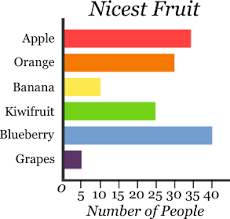
\includegraphics[width=.5\textwidth]{./figures/query1}
\caption{Results for BI Query 1}
\label{fig:query1}
\end{figure}

%% ===============================
\subsection{BI Query 2: \ldots}
\label{sec:BITwo}
%% ===============================

For this query, the contributing sources of data are: \ldots

The general findings are that \ldots as illustrated in \figurename~\ref{fig:query1}.

\begin{figure}[ht]
\centering
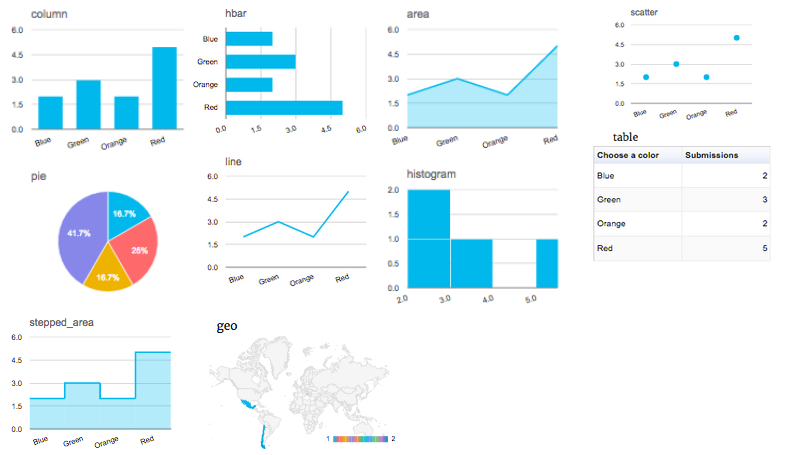
\includegraphics[width=.75\textwidth]{./figures/dashboard}
\caption{Results for BI Query 2}
\label{fig:query2}
\end{figure}

%% ===============================
\subsection{BI Query 3: \ldots}
\label{sec:BIThree}
%% ===============================

For this query, the contributing sources of data are: \ldots

The general findings are that \ldots as illustrated in \figurename~\ref{fig:query1}.

\begin{figure}[ht]
\centering
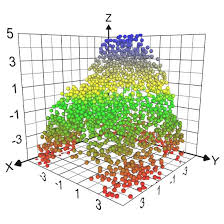
\includegraphics[width=.5\textwidth]{./figures/query3}
\caption{Results for BI Query 3}
\label{fig:query3}
\end{figure}

%% ===============================
\subsection{Discussion}
\label{sec:discussion}
%% ===============================

A detailed discussion / summarisation of the findings from the 3 queries. Note that this discussion will have a lot more detail than the discussion in the following section (Conclusion). You should relate your main findings to the literature that you reviewed in Section~\ref{sec:rw}, i.e. those with a similar topic to your data warehousing project (but which are not necessarily data warehousing projects), and compare and contrast your findings with theirs. 
%% conclusion.tex
%%

%% ==================
\section{Conclusion and Future Work}
\label{sec:Conclusion}
%% ==================

(Partially) answer your research question and discuss the implications of your (partial) answer, talk about the efficacy of your research, and discuss its limitations. 

\dots

Present \textbf{MEANINGFUL} future work. Sweeping more parameters in your simulation / model / platform is probably not meaningful. More discuss what could a follow up research project do, to better / differently approach / extend etc. your work.



%% --------------------
%% |   Bibliography   |
%% --------------------

% Style
\bibliographystyle{agsm}
\bibliography{refs}


%% --------------------
%% |   Appendix   |
%% --------------------
\section*{Appendix}

\subsection*{R code example}

\begin{lstlisting}
#Calculate CE for each counterparty
Value.A <- data.frame() #MTM value of each contract within cp A
# ...
for(i in 1:length(foo)){
  if(isTrue(as.character(portfolio_data[i,1])=="A")==TRUE){
    # ...
  }
}
\end{lstlisting}

\end{document}
